\documentclass[preprint,12pt,sort&compress]{elsarticle}

\usepackage[T1]{fontenc}
\usepackage[utf8]{inputenc}
\usepackage{amsmath,amssymb,amsfonts,mathtools}
\usepackage{amsthm}
\usepackage{graphicx}
\usepackage{booktabs}
\usepackage{array}
\usepackage{tabularx}
\usepackage{multirow}
\usepackage{enumitem}
\usepackage{url}
\usepackage{xcolor}
\usepackage{hyperref}
\hypersetup{colorlinks=true, linkcolor=blue, citecolor=blue, urlcolor=blue}
\pdfstringdefDisableCommands{\def\corref#1{}\def\cnoteref#1{}}

\journal{Computer Methods in Applied Mechanics and Engineering}

\newtheorem{definition}{Definition}
\newtheorem{assumption}{Assumption}
\newtheorem{proposition}{Proposition}
\newtheorem{lemma}{Lemma}
\newtheorem{theorem}{Theorem}
\newtheorem{remark}{Remark}

\newcommand{\R}{\mathbb{R}}
\newcommand{\dd}{\mathrm{d}}
\newcommand{\dist}{\operatorname{dist}}
\newcommand{\cone}{\operatorname{cone}}
\newcommand{\conv}{\operatorname{conv}}
\newcommand{\diag}{\operatorname{diag}}
\newcommand{\argmin}{\operatorname*{arg\,min}}
\newcommand{\argmax}{\operatorname*{arg\,max}}
\newcommand{\norm}[1]{\left\lVert #1 \right\rVert}
\newcommand{\abs}[1]{\left\lvert #1 \right\rvert}
\newcommand{\ip}[2]{\left\langle #1,#2 \right\rangle}
\newcommand{\T}{\mathsf{T}}
\newcommand{\Id}{\mathbf{I}}
\newcommand{\cO}{\mathcal{O}}
\newcommand{\cM}{\mathcal{M}}
\newcommand{\cN}{\mathcal{N}}
\newcommand{\cF}{\mathcal{F}}
\newcommand{\cC}{\mathcal{C}}
\newcommand{\cA}{\mathcal{A}}
\newcommand{\cL}{\mathcal{L}}
\newcommand{\cR}{\mathcal{R}}
\newcommand{\cQ}{\mathcal{Q}}
\newcommand{\cJ}{\mathcal{J}}
\newcommand{\cP}{\mathcal{P}}
\newcommand{\cB}{\mathcal{B}}
\newcommand{\cV}{\mathcal{V}}
\newcommand{\cT}{\mathcal{T}}
\newcommand{\eps}{\varepsilon}

\begin{document}
\emergencystretch=3em

\begin{frontmatter}

\title{A Feature-Aware Contact-SDF Atlas for Fast and Consistent Contact Geometry Queries from Corner-Normal Triangle Meshes}

\author[inst1]{Sohansome Body\corref{cor1}}
\ead{author@example.com}
\author[inst1]{Second Author}
\author[inst2]{Third Author}
\cortext[cor1]{Corresponding author. This is a manuscript draft; author names, e-mail addresses, affiliations, funding information and declarations should be edited before submission.}

\address[inst1]{Department of Mechanical Engineering, Institution, City, Country}
\address[inst2]{Department of Computational Mechanics, Institution, City, Country}

\begin{abstract}
Signed distance fields (SDFs) are attractive for contact simulation because they support constant-time geometric queries after preprocessing. However, differentiating an interpolated scalar SDF generally yields contact normals and curvatures that depend on the interpolation basis rather than on the underlying geometry. Conversely, closest-point projection provides geometrically consistent contact quantities but is often too expensive to solve repeatedly in multibody and finite element time stepping. This paper proposes a feature-aware Contact-SDF Atlas for corner-normal triangle meshes, a common engineering format in which each triangle stores three positions and three face-corner normals. The method interprets discontinuous corner normals as normal sectors, builds local smooth and multi-sector contact records, and moves closest-feature computation from runtime to offline atlas construction. Smooth atlas leaves store local signed-distance jets with gap, normal and optional Hessian information, whereas nonsmooth edge and vertex leaves store active normal-sector records and normal cones. A feature-specific adaptive refinement strategy concentrates resolution near normal-sector transitions without globally increasing the SDF resolution. The resulting query interface returns contact-ready gap, normal, optional Hessian and multi-normal constraints without online projection. Benchmarks on analytically generated ellipsoids, prisms and cones show that the atlas reduces contact-normal error relative to trilinear and tricubic scalar SDFs; a compact batch query backend separates the higher offline construction cost from sub-microsecond runtime lookup in the Python prototype. The formulation is solver-agnostic and can be coupled to penalty, augmented-Lagrangian, LCP/NCP or variational contact solvers.
\end{abstract}

\begin{keyword}
contact mechanics \sep signed distance fields \sep corner-normal meshes \sep normal cones \sep closest-point projection \sep multibody dynamics
\end{keyword}

\end{frontmatter}

\section*{Highlights}
\begin{itemize}[leftmargin=1.5em]
\item Corner-normal meshes are converted into normal-sector contact geometry.
\item The atlas stores contact jets and normal cones, not scalar samples.
\item Feature-specific refinement targets sharp edges and vertices.
\item Runtime contact queries avoid closest-point projection.
\item Benchmarks show improved normals and 9.9--10.7x speedups.
\end{itemize}

\section{Introduction}
\label{sec:introduction}

Contact simulation requires geometric information that is more stringent than the information needed for visualization or collision culling. A contact solver usually needs at least a gap function, a contact normal and a mapping of the contact constraint to the generalized coordinates. Higher-order methods, implicit time stepping, stiffness linearization and curvature-aware regularization may additionally require a consistent Hessian of the gap function. In many engineering pipelines, however, the contact geometry is supplied as a tessellated boundary mesh rather than as an analytic or CAD boundary representation. Commercial multibody dynamics tools and model-exchange formats frequently store a triangle mesh together with local normals at the three corners of each triangle. Such data will be called a \emph{corner-normal triangle mesh} in this paper. The same geometric vertex may have several different normals in adjacent triangles; this is not a data error but a compact way of encoding smooth charts, sharp edges and normal discontinuities.

Signed distance fields (SDFs) are a natural candidate for accelerating contact geometry. A scalar SDF sampled on a regular or sparse grid gives a fast query for the signed gap, and modern volume data structures make it possible to store narrow-band distance data compactly. The standard approach is to interpolate the scalar values and then compute the contact normal as the gradient of the interpolant. This is fast, but it creates a fundamental mismatch: the computed normal and Hessian are derivatives of a chosen interpolation basis, not necessarily derivatives of the original geometric boundary. A trilinear SDF has discontinuous gradients at cell boundaries and an almost meaningless cellwise Hessian. Tricubic, radial-basis or neural fields provide smoother derivatives, but their derivatives are still derivatives of an approximate field. For contact mechanics this distinction matters because normal errors directly enter contact forces, impulses, constraint Jacobians and stiffness matrices.

Closest-point projection is the opposite extreme. Given a query point, one solves a local minimization problem on the contact surface, obtains the closest point, and derives the signed gap and normal from the geometry itself. The projection viewpoint is classical in contact mechanics and is essential in high-order and isogeometric contact formulations \cite{Konyukhov2008,Lu2011,Temizer2011}. Its difficulty is cost and robustness. Repeatedly solving closest-point problems during contact detection, nonlinear iterations or time stepping can dominate the runtime, especially for many contact candidates. The projection may also be nonunique near sharp edges, vertices or the medial axis. In these locations the signed distance itself is nonsmooth; enforcing a single smoothed normal is often less physical than preserving the active normal cone.

This work proposes a representation that combines the speed of SDF lookup with contact quantities closer to those obtained from projection. The key idea is to avoid storing only scalar samples. Instead, we build a \emph{Contact-SDF Atlas}: a sparse adaptive narrow-band atlas whose leaves store local contact records. Smooth leaves contain a local signed-distance jet, e.g. a Taylor model with gap, normal and optional Hessian. Nonsmooth leaves contain active normal-sector records and a discrete normal cone. The expensive closest-feature computation is performed during preprocessing and is then compressed into leaf records. Runtime evaluation becomes a cell lookup and a low-order polynomial or multi-plane evaluation.

The method is designed for corner-normal meshes, but the abstraction is more general. Any source that can provide local surface positions, normal sectors and feature adjacency can be used: an analytic primitive can be sampled into the same form, a CAD boundary representation can be tessellated while preserving face normals and trim features, a high-order finite element boundary can provide curved patch derivatives, and a plain triangle mesh can fall back to face normals. This makes the proposed atlas a geometry backend rather than a specific contact law. It can supply contact quantities to penalty, augmented-Lagrangian, linear complementarity, nonlinear complementarity, nonsmooth time-stepping or variational contact solvers.

The main contributions are:
\begin{enumerate}[label=(\arabic*), leftmargin=1.8em]
\item A normal-sector interpretation of corner-normal triangle meshes, preserving multiple normals at the same geometric position instead of averaging them into a single vertex normal.
\item A feature-aware Contact-SDF Atlas that stores contact-ready records rather than scalar SDF samples: smooth signed-distance jets on smooth charts and normal-cone records at sharp features.
\item A theoretical derivation of smooth local SDF jets from closest-point geometry and of nonsmooth contact records from active normal sectors.
\item A feature-specific adaptive refinement strategy that refines edge, vertex and multi-sector leaves more deeply than smooth leaves.
\item A solver-agnostic query interface returning gap, normal, optional Hessian and active normal constraints without online closest-point projection.
\item A prototype validation on analytic smooth and nonsmooth geometries showing improved contact-normal consistency compared with scalar trilinear and tricubic SDFs, together with separated offline construction and compact runtime-query measurements.
\end{enumerate}

The remainder is organized as follows. Section~\ref{sec:related} discusses related work. Section~\ref{sec:problem} defines the corner-normal contact geometry. Section~\ref{sec:smooth} derives the smooth signed-distance jet. Section~\ref{sec:nonsmooth} treats nonsmooth features and normal cones. Section~\ref{sec:atlas} defines the Contact-SDF Atlas and the adaptive refinement algorithm. Section~\ref{sec:solver} describes coupling to contact solvers. Section~\ref{sec:numerical} presents validation results. Section~\ref{sec:discussion} discusses generality and limitations.

\section{Related work}
\label{sec:related}

\subsection{Closest-point projection and computational contact mechanics}

Frictionless contact formulations typically rely on a normal gap function and a contact normal derived from a closest-point or closest-feature relation \cite{Wriggers2006,Laursen2002}. Konyukhov and Schweizerhof analyzed the existence and uniqueness of closest-point projection procedures for surfaces of arbitrary geometry and emphasized that edges and vertices must be treated explicitly when surfaces are not globally smooth \cite{Konyukhov2008,Konyukhov2013}. Isogeometric contact formulations exploit the availability of smooth NURBS geometry to compute consistent normal gaps, tangents and curvature terms \cite{Lu2011,Temizer2011}. These approaches motivate our use of closest-point geometry for contact quantities. The difference is that we do not leave the projection problem as a runtime operation; we precompute and store local contact records in an atlas.

\subsection{Signed distance fields}

Level-set and signed-distance methods provide a powerful implicit representation for evolving and querying shapes \cite{Sethian1999,OsherFedkiw2003}. In geometry processing and graphics, adaptively sampled distance fields and sparse volume data structures have been developed to compactly represent high-resolution distance information \cite{Frisken2000,Museth2013}. Higher-order and hp-adaptive SDFs improve scalar field approximation by fitting polynomial representations on adaptive cells \cite{Koschier2017,Pujol2023}. These methods increase the accuracy of the field, but the contact normal remains a derivative of the stored scalar approximation unless additional geometric information is retained. Our contribution is not another scalar SDF approximation. The atlas stores contact semantics: feature identifiers, normal sectors, local SDF jets and normal cones.

SDF-based contact has also been used for granular media and arbitrary particles. For example, SDF-DEM frameworks define an SDF function and a surface projection function to handle particles with arbitrary shapes \cite{Lai2022}. These methods show the usefulness of implicit geometry for contact operations. The present work focuses on a different bottleneck: how to avoid both interpolated-gradient artifacts and repeated runtime projection when the input is a corner-normal engineering mesh.

\subsection{Primitive-based and variational contact}

Primitive-based collision and contact formulations operate on point-triangle, edge-edge and related pairs. Incremental Potential Contact (IPC) provides a robust variational framework for intersection- and inversion-free dynamics \cite{Li2020IPC}; high-order IPC extends the idea to curved meshes and high-order finite elements \cite{Ferguson2023}. These methods are complementary to the proposed atlas. IPC defines a contact potential and a robust solver strategy. The Contact-SDF Atlas is instead a contact-geometry oracle that can supply gap and normal information to multiple solvers. It is particularly useful when the same rigid or quasi-rigid body is queried many times and when the mesh carries corner-normal information that should not be discarded.

\subsection{Normals, curved triangles and sharp features}

Point-normal patches, such as PN triangles, show that triangle vertices and normals can be used to reconstruct a local curved surface proxy \cite{Vlachos2001}. Such reconstruction is valuable on smooth charts, but it is unsafe across sharp features. Mesh processing literature distinguishes geometric vertices from normal or texture seams; averaging normals across a hard edge destroys the intended feature \cite{Botsch2010}. The proposed normal-sector complex follows this principle in a contact context: positions may be welded for topology, but face-corner normals remain separate and define sectors.

\subsection{Nonsmooth contact and normal cones}

At sharp features, a unique smooth normal does not exist. Nonsmooth analysis describes contact reactions through normal cones and subdifferentials \cite{Clarke1983,Moreau1988}. Time-stepping schemes for rigid-body dynamics similarly use complementarity and cone constraints to represent unilateral contact and friction \cite{StewartTrinkle1996,AnitescuPotra1997}. Our nonsmooth atlas leaves store finite normal-sector cones, so a downstream solver can activate multiple local constraints instead of receiving a single averaged normal.

\section{Problem setting and corner-normal contact geometry}
\label{sec:problem}

\subsection{Input representation}

The basic input is a set of oriented triangle records
\begin{equation}
T_f = \left(x_{f0},x_{f1},x_{f2}; n_{f0},n_{f1},n_{f2}\right),
\qquad f=1,\ldots,N_f,
\label{eq:corner_record}
\end{equation}
where $x_{fi}\in\R^3$ is the position of the $i$th corner of triangle $f$, and $n_{fi}\in\mathbb{S}^2$ is the corresponding corner normal. The same geometric coordinate may occur in several triangles with different normals. We therefore distinguish between a \emph{geometric vertex}, obtained by welding positions within a tolerance, and a \emph{corner}, indexed by $(f,i)$.

The geometric triangle normal is
\begin{equation}
 m_f = \frac{(x_{f1}-x_{f0})\times (x_{f2}-x_{f0})}{\norm{(x_{f1}-x_{f0})\times (x_{f2}-x_{f0})}}.
\end{equation}
Corner normals are normalized and, if needed, flipped consistently with the global orientation. The input normals are not assumed to be exact differential geometry. They are treated as contact-relevant local normal sectors. Their discontinuities are preserved.

\begin{definition}[Corner-normal mesh]
A corner-normal mesh is a tuple
\begin{equation}
 \cM_N = (\cV_g,\cT,\cC, X, N),
\end{equation}
where $\cV_g$ is the welded geometric-vertex set, $\cT$ is the triangle set, $\cC=\{(f,i)\}$ is the set of face corners, $X:\cC\to\R^3$ maps each corner to its position and $N:\cC\to\mathbb{S}^2$ maps each corner to its normal.
\end{definition}

This representation includes several common cases. If the mesh is a standard vertex-normal mesh, all corners incident to a geometric vertex may share the same normal. If the mesh is a faceted STL, each corner normal can be set to the face normal. If the mesh is produced from CAD or an engineering solver, different normals at the same position can represent smooth charts meeting at sharp edges.

\subsection{Normal sectors}

Let $\cC(v)=\{(f,i)\in\cC: X(f,i)=x_v\}$ be the corners incident to a welded geometric vertex $v$. A single averaged normal at $v$ is not used. Instead, the incident corner normals are clustered into sectors.

\begin{definition}[Normal sector]
For a geometric vertex $v$, define a graph $G_v$ with node set $\cC(v)$. Two nodes $(f,i)$ and $(g,j)$ are connected if they are topologically adjacent through a mesh edge or face fan and
\begin{equation}
 \arccos \left(N(f,i)^\T N(g,j)\right) \leq \theta_s,
\label{eq:sector_threshold}
\end{equation}
where $\theta_s$ is a smooth-sector tolerance. The connected components of $G_v$ are the normal sectors at $v$.
\end{definition}

The sector representative may be the normalized average of normals inside the component. The tolerance $\theta_s$ is not a physical contact parameter; it is a preprocessing parameter that interprets the exported corner normals. A second threshold $\theta_h>\theta_s$ can be used to mark ambiguous cases for refinement.

\subsection{Smooth charts and sharp features}

A mesh edge shared by triangles $f$ and $g$ has two endpoints $a$ and $b$. Let the corresponding corner normals on the two sides be $n_{f,a},n_{g,a}$ and $n_{f,b},n_{g,b}$. Define the corner-normal jumps
\begin{equation}
\theta_a = \arccos(n_{f,a}^\T n_{g,a}), \qquad
\theta_b = \arccos(n_{f,b}^\T n_{g,b}).
\end{equation}
The edge is classified as smooth if $\theta_a,\theta_b\leq \theta_s$ and as sharp if at least one jump exceeds $\theta_h$. Between the two thresholds the edge is ambiguous and is treated conservatively as a multi-sector feature unless refinement resolves it.

Connected components of triangles across smooth edges form smooth charts $C_k$. Sharp edges and sharp vertices form lower-dimensional features. Thus the input boundary is treated as a discrete stratified complex
\begin{equation}
 \Gamma_h = \left(\bigcup_k C_k\right) \cup \left(\bigcup_j E_j\right) \cup \left(\bigcup_l V_l\right),
\label{eq:stratified}
\end{equation}
where $C_k$ are two-dimensional smooth charts, $E_j$ are one-dimensional normal-sector discontinuities and $V_l$ are zero-dimensional corner features.

This distinction is essential. A smooth chart can support a local differentiable distance model. A sharp edge or vertex cannot be faithfully represented by a single normal and Hessian. At such features the correct object for frictionless contact is a normal cone.

\subsection{Contact query objective}

For a body occupying $\Omega\subset\R^3$ with boundary $\Gamma=\partial\Omega$, the exact signed distance is
\begin{equation}
 \phi(x) = s(x) \inf_{y\in\Gamma} \norm{x-y},
\label{eq:exact_sdf}
\end{equation}
where $s(x)$ is the sign convention. In an ideal smooth neighborhood, the closest point is unique and the distance is differentiable. For a corner-normal mesh, the exact object being represented is not a globally smooth SDF. The contact query should instead return
\begin{equation}
 \cQ(x)=\{g,p,\mathrm{mode},\mathrm{feature}, n, H, \{(g_i,n_i)\}_{i=1}^m, N, \epsilon\},
\label{eq:query_object}
\end{equation}
where $g$ is a scalar gap used for sorting or smooth contact, $p$ is a closest or representative contact point, $n$ and $H$ are valid only in smooth mode, $\{(g_i,n_i)\}$ and $N$ are used in nonsmooth mode, and $\epsilon$ is an error or validity indicator.

The goal of the Contact-SDF Atlas is to approximate the query map $\cQ$ by storing local records on a sparse adaptive partition of a narrow band around $\Gamma_h$.

\section{Smooth closest-point SDF jets}
\label{sec:smooth}

This section derives the local SDF jet stored in smooth atlas leaves. The derivation is standard differential geometry but is included to make clear that the desired normal and Hessian are geometry-induced quantities, not interpolation artifacts.

\subsection{Closest-point projection on a smooth chart}

Let $r:U\subset\R^2\to\R^3$ be a $C^k$ parameterization, $k\geq 3$, of a smooth chart, with tangent vectors $r_1=\partial r/\partial u^1$ and $r_2=\partial r/\partial u^2$. The unit normal is
\begin{equation}
 n = \frac{r_1\times r_2}{\norm{r_1\times r_2}}.
\end{equation}
For a query point $x$ sufficiently close to the chart, the closest-point projection solves
\begin{equation}
 u^*(x) = \argmin_{u\in U} \frac{1}{2}\norm{x-r(u)}^2.
\label{eq:projection}
\end{equation}
The first-order optimality conditions are
\begin{equation}
 r_\alpha(u^*)^\T\left(x-r(u^*)\right)=0, \qquad \alpha=1,2.
\label{eq:orthogonality}
\end{equation}
If the closest point is unique and lies in the chart interior, the vector $x-r(u^*)$ is normal to the chart. We write
\begin{equation}
 x = r(u^*) + d n(u^*), \qquad d=\phi(x).
\label{eq:normal_coordinate}
\end{equation}

\begin{assumption}[Tubular validity]
\label{ass:tubular}
The smooth chart has a unique closest-point projection in the neighborhood of interest, the projection lies away from the chart boundary, and the normal-coordinate map
\begin{equation}
 \Psi(u,d)=r(u)+d n(u)
\end{equation}
remains locally invertible.
\end{assumption}

This assumption fails near sharp features, trim boundaries or the medial axis. Those cases are handled by nonsmooth records rather than smooth jets.

\subsection{Gradient and Hessian of the signed distance}

Let $P_T=\Id-n\otimes n$ be the tangent projector. We use the shape-operator convention
\begin{equation}
 S\tau = -D_\tau n, \qquad \tau\in T_p\Gamma.
\label{eq:shape_operator}
\end{equation}
For a sphere with outward normal this convention gives negative principal curvatures. Let $\kappa_a$ and $e_a$, $a=1,2$, be the eigenpairs of $S$.

\begin{proposition}[Smooth SDF derivatives]
\label{prop:sdf_derivatives}
Under Assumption~\ref{ass:tubular}, the signed distance satisfies
\begin{equation}
 \nabla_x \phi(x)=n(p), \qquad p=r(u^*(x)),
\label{eq:grad_phi}
\end{equation}
and its Hessian is
\begin{equation}
 \nabla_x^2\phi(x) = -S(I-dS)^{-1}P_T.
\label{eq:hessian_operator}
\end{equation}
In principal directions this is
\begin{equation}
 \nabla_x^2\phi(x) = \sum_{a=1}^2 \frac{-\kappa_a}{1-d\kappa_a}\, e_a\otimes e_a,
\label{eq:hessian_principal}
\end{equation}
with zero eigenvalue in the normal direction.
\end{proposition}

\begin{proof}
Differentiating the normal-coordinate map gives, for a tangent direction $\tau$ at the surface,
\begin{equation}
 D\Psi[\tau] = \tau + d D_\tau n = (I-dS)\tau,
\end{equation}
and $D\Psi[n]=n$ in the normal direction. Therefore a spatial tangent displacement at the offset surface corresponds to a surface tangent displacement through $(I-dS)^{-1}$. Since $\phi(r(u)+dn(u))=d$, its derivative in the normal direction is one and in offset tangential directions is zero; hence $\nabla\phi=n$. Differentiating $n$ with respect to a spatial tangent displacement gives $D n = -S(I-dS)^{-1}P_T$, which is the Hessian of $\phi$. The principal-direction form follows by diagonalizing $S$.
\end{proof}

Equation~\eqref{eq:hessian_principal} shows why an SDF Hessian should be a curvature quantity. It is not generally reproduced by differentiating a trilinear or tricubic grid field. For example, for a sphere of radius $R$ and outward signed distance $d=\norm{x-c}-R$, the convention above gives $\kappa_1=\kappa_2=-1/R$ and Eq.~\eqref{eq:hessian_principal} yields
\begin{equation}
 \nabla^2\phi = \frac{1}{R+d}(\Id-n\otimes n),
\end{equation}
which is the analytic result.

\subsection{Local Taylor jet}

Let $x_L$ be a leaf center in a smooth atlas leaf and let
\begin{equation}
 \phi_L=\phi(x_L),\qquad n_L=\nabla\phi(x_L),\qquad H_L=\nabla^2\phi(x_L).
\end{equation}
The second-order signed-distance jet is
\begin{equation}
 \widehat{\phi}_L(x)=\phi_L+n_L^\T\Delta x+\frac{1}{2}\Delta x^\T H_L\Delta x,
 \qquad \Delta x=x-x_L.
\label{eq:second_order_jet}
\end{equation}
The associated gradient and Hessian are
\begin{equation}
 \widehat{n}_L(x)=\nabla\widehat\phi_L(x)=n_L+H_L\Delta x,
 \qquad \widehat H_L(x)=H_L.
\label{eq:jet_gradient}
\end{equation}
The normal returned to a contact solver is $\widehat n_L/\norm{\widehat n_L}$.

A third-order record can also be stored:
\begin{equation}
 \widehat{\phi}_L^{(3)}(x)=\phi_L+n_L^\T\Delta x+\frac{1}{2}\Delta x^\T H_L\Delta x
 +\frac{1}{6}T_L[\Delta x,\Delta x,\Delta x],
\label{eq:third_order_jet}
\end{equation}
where $T_L=\nabla^3\phi(x_L)$. In practice, the second-order jet already captures curvature effects important for contact normals and linearization, while the third-order tensor increases storage. The prototype in Section~\ref{sec:numerical} therefore uses second-order smooth records.

\subsection{Jet error estimates}

Let $B_L$ be a leaf with radius $h_L$ and assume $\phi\in C^3(B_L)$. If
\begin{equation}
 M_{3,L}=\sup_{x\in B_L}\norm{\nabla^3\phi(x)},
\end{equation}
then Taylor's theorem gives
\begin{align}
 \abs{\phi(x)-\widehat\phi_L(x)} &\leq \frac{M_{3,L}}{6}\norm{x-x_L}^3,\label{eq:error_phi}\\
 \norm{\nabla\phi(x)-\nabla\widehat\phi_L(x)} &\leq \frac{M_{3,L}}{2}\norm{x-x_L}^2,\label{eq:error_grad}\\
 \norm{\nabla^2\phi(x)-H_L} &\leq M_{3,L}\norm{x-x_L}.\label{eq:error_hessian}
\end{align}
These estimates justify refining high-curvature regions and using smooth jets only where a unique projection and bounded curvature derivatives are credible. For a third-order record, analogous estimates use $\nabla^4\phi$ and yield one order higher accuracy for the scalar field.

\section{Nonsmooth feature records and normal cones}
\label{sec:nonsmooth}

\subsection{Why a single SDF jet is inappropriate at sharp features}

At a sharp edge or vertex, the boundary is not a $C^2$ manifold. Even when the signed distance exists as a scalar function, it may not be differentiable because the closest point or the normal direction is not unique. A grid or neural SDF can produce a smooth field, but such smoothness is a regularization of the geometry, not a property of the original contact set. In contact mechanics, the reaction at a sharp convex feature may lie anywhere in the normal cone spanned by adjacent smooth-sector normals.

Consider a sharp edge shared by two smooth charts with outward normals $n_1$ and $n_2$. The local normal cone is approximated by
\begin{equation}
 N_E = \cone\{n_1,n_2\}=\{\lambda_1 n_1+\lambda_2 n_2:\lambda_1,\lambda_2\geq0\}.
\label{eq:edge_cone}
\end{equation}
At a vertex with incident normals $n_1,\ldots,n_m$,
\begin{equation}
 N_V = \cone\{n_1,\ldots,n_m\}.
\label{eq:vertex_cone}
\end{equation}
Averaging these normals into one direction can create an artificial fillet and may produce a reaction direction outside the physically admissible cone for nonconvex configurations.

\subsection{Finite normal-sector constraints}

In a nonsmooth atlas leaf, we store a set of local sector gap models
\begin{equation}
 g_{i,L}(x)=\phi_{i,L}+n_{i,L}^\T\Delta x + \frac{1}{2}\Delta x^\T H_{i,L}\Delta x,
 \qquad i=1,\ldots,m_L,
\label{eq:sector_gap_model}
\end{equation}
where $H_{i,L}$ may be omitted or set to zero for first-order feature planes. The nonsmooth contact mode returns the active set
\begin{equation}
 \cA_L=\{(g_{i,L},n_{i,L})\}_{i=1}^{m_L}, \qquad N_L=\cone\{n_{i,L}:i=1,\ldots,m_L\}.
\label{eq:active_set_record}
\end{equation}
A scalar value may still be returned for broad sorting, e.g.
\begin{equation}
 g_L^{\min}(x)=\min_{i=1,\ldots,m_L} g_{i,L}(x),
\end{equation}
whereas the contact solver receives all active constraints. For a frictionless complementarity formulation this gives
\begin{equation}
 0\leq \lambda_i \perp g_{i,L}(q)\geq 0, \qquad
 f_c = \sum_{i=1}^{m_L}\lambda_i n_{i,L},
\label{eq:multi_complementarity}
\end{equation}
so that the resultant force lies in the discrete normal cone.

\begin{remark}
The stored normal cone is a discrete approximation of the geometric normal cone induced by the input normal sectors. If the input mesh came from a CAD model with correct feature normals, the cone is a faithful representation of the tessellated CAD feature. If the input normals are visual normals or are noisy, the cone represents the provided data and should be validated or regularized during preprocessing.
\end{remark}

\section{Contact-SDF Atlas}
\label{sec:atlas}

\subsection{Narrow-band atlas domain}

Let $\Gamma_h$ be the stratified corner-normal mesh complex. The atlas is built in a narrow band
\begin{equation}
 \cB_w = \{x\in\R^3: \dist(x,\Gamma_h)\leq w\},
\end{equation}
where $w$ is chosen from the expected maximum contact search radius, penetration allowance or clearance tolerance. Outside the band, a broadphase structure such as a bounding-volume hierarchy can be used.

The band is partitioned into leaves $L\in\cL$. A leaf may be a uniform grid cell, an octree cell or a sparse blocked-grid cell. Each leaf stores a record
\begin{equation}
 \cR_L = (\mathrm{mode}_L, x_L, h_L, \mathrm{data}_L, \epsilon_L),
\end{equation}
where $x_L$ is the leaf center and $h_L$ is a leaf radius. The mode is one of
\begin{equation}
 \mathrm{mode}_L\in\{\mathrm{smooth},\mathrm{edge},\mathrm{vertex},\mathrm{multi},\mathrm{invalid}\}.
\end{equation}

\begin{definition}[Contact-SDF Atlas]
A Contact-SDF Atlas is a tuple
\begin{equation}
 \cA_h = (\cL, \mathcal{I}, \{\cR_L\}_{L\in\cL}),
\end{equation}
where $\cL$ is an adaptive leaf partition of $\cB_w$, $\mathcal{I}$ is a lookup map from spatial coordinates to leaf indices, and $\cR_L$ is a contact record. A smooth record stores $\phi_L,n_L,H_L$ and optional $T_L$; a nonsmooth record stores a finite set of sector gap models and the corresponding normal cone.
\end{definition}

The lookup map $\mathcal I$ can be implemented by a finest-level indirection table for dyadic octrees, by a sparse hash map for block grids, or by a VDB-style hierarchical tree. In all cases, the runtime operation is a lookup plus record evaluation rather than a closest-point solve.

\subsection{Offline construction}

The offline construction uses accurate, possibly expensive, feature queries. For each candidate leaf $L$, one samples a finite set of points $\cP_L$ such as the center, vertices and face centers. For each sample point, a reference query is performed against the normal-sector complex. This reference may use a triangle BVH and local point-to-triangle projection, PN-triangle projection in smooth charts, CAD projection if a CAD kernel is available, or analytic projection for analytic primitives.

The active feature set over $\cP_L$ is then inspected:
\begin{itemize}[leftmargin=1.6em]
\item if all samples have the same smooth chart as the active feature and the projection is far from chart boundaries, a smooth jet record is fitted or sampled at $x_L$;
\item if samples compete between adjacent normal sectors, the leaf becomes an edge or multi-sector record;
\item if several sectors meet at a welded vertex, the leaf becomes a vertex record;
\item if the feature state is unstable or the error estimate is too large, the leaf is subdivided.
\end{itemize}

The following abstract pseudocode summarizes the construction.

\begin{figure}[htbp]
\small
\begin{tabularx}{\textwidth}{@{}lX@{}}
\toprule
\multicolumn{2}{@{}l}{\textbf{Algorithm 1. Feature-aware Contact-SDF Atlas construction}}\\
\midrule
1 & Read corner-normal triangle records $T_f=(x_{f0},x_{f1},x_{f2};n_{f0},n_{f1},n_{f2})$.\\
2 & Weld positions to form geometric vertices; keep all face-corner normals separate.\\
3 & Build normal sectors at welded vertices using Eq.~\eqref{eq:sector_threshold}.\\
4 & Classify mesh edges as smooth, sharp or ambiguous; build smooth charts.\\
5 & Initialize a narrow-band root partition around $\Gamma_h$.\\
6 & For each candidate leaf $L$, evaluate reference feature queries at samples $\cP_L$.\\
7 & If $L$ is smooth and error/certificates pass, store $\phi_L,n_L,H_L$.\\
8 & Else if $L$ contains edge/vertex/multi-sector behavior, store active sector models and a normal cone.\\
9 & If error is too large or feature state is unstable, subdivide $L$.\\
10 & Permit deeper subdivision for edge/vertex/multi-sector leaves than for smooth leaves.\\
11 & Build the runtime lookup map $\mathcal I$ from finest grid keys to leaf records.\\
\bottomrule
\end{tabularx}
\caption{Offline atlas construction. The expensive closest-feature operations occur in steps 6--8 and are not executed at runtime.}
\label{alg:construction}
\end{figure}

\subsection{Runtime evaluation}

Given a query point $x$, the atlas returns
\begin{equation}
 L=\mathcal I(x), \qquad \Delta x=x-x_L.
\end{equation}
If $L$ is smooth, the runtime evaluation uses Eq.~\eqref{eq:second_order_jet} or Eq.~\eqref{eq:third_order_jet}. If $L$ is nonsmooth, each stored sector model Eq.~\eqref{eq:sector_gap_model} is evaluated. No global feature search or iterative projection is performed.

\begin{figure}[htbp]
\centering
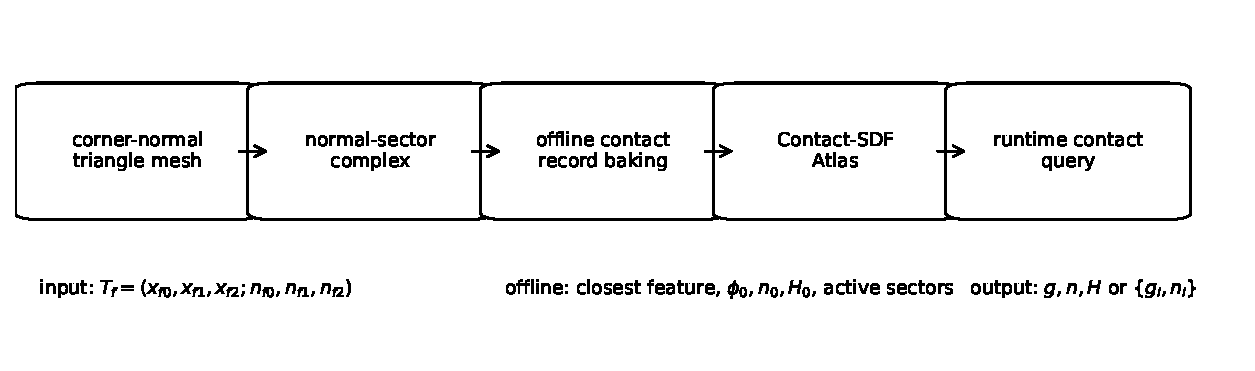
\includegraphics[width=0.95\textwidth]{fig_pipeline.pdf}
\caption{Conceptual pipeline. The corner-normal mesh is converted to a normal-sector complex. Closest-feature computation is moved to offline atlas construction. Runtime contact queries evaluate stored smooth jets or normal-cone records.}
\label{fig:pipeline}
\end{figure}

\begin{figure}[htbp]
\centering
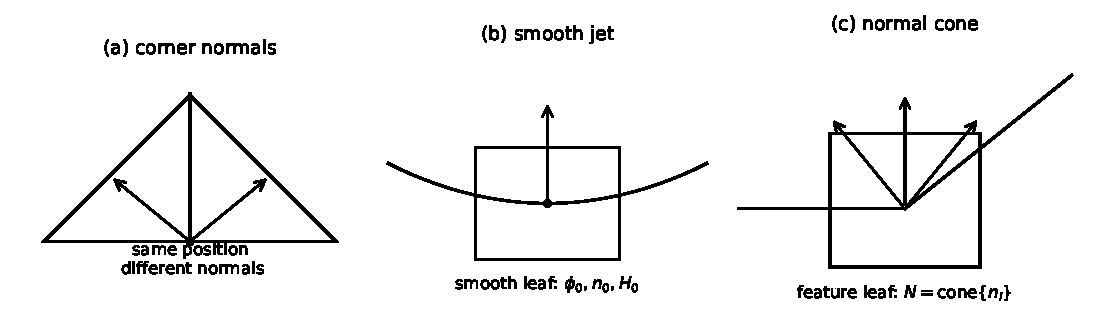
\includegraphics[width=0.95\textwidth]{fig_leaf_types.pdf}
\caption{Normal-sector interpretation and leaf records. (a) The same geometric position can carry different face-corner normals. (b) Smooth leaves store a local SDF jet. (c) Sharp leaves store an active normal cone rather than an averaged normal.}
\label{fig:leaf_types}
\end{figure}

\subsection{Feature-specific adaptive refinement}

Uniform refinement is inefficient because most cells in a narrow band lie over smooth regions where the SDF is well approximated by a low-order jet. The difficult regions are normal-sector transitions, sharp edges, vertices and ambiguous active-feature zones. We therefore use two depth limits:
\begin{equation}
 d_{\max}^{\mathrm{smooth}} \leq d_{\max}^{\mathrm{feature}}.
\end{equation}
Smooth cells are refined until the Taylor error or normal error passes the tolerance or until $d_{\max}^{\mathrm{smooth}}$ is reached. Feature cells may continue to $d_{\max}^{\mathrm{feature}}$. This concentrates storage around nonsmooth contact-relevant regions.

A cell $L$ is refined if any of the following indicators is triggered:
\begin{align}
 \eta_g(L) &= \max_{x\in\cP_L} \abs{\phi_{\mathrm{ref}}(x)-\widehat\phi_L(x)} > \tau_g,\\
 \eta_n(L) &= \max_{x\in\cP_L} \angle(n_{\mathrm{ref}}(x),\widehat n_L(x)) > \tau_n,\\
 \eta_f(L) &= 1 \quad \text{if more than one normal sector is active on }\cP_L,\\
 \eta_b(L) &= 1 \quad \text{if a projected point lies near a chart boundary.}
\end{align}
The feature-specific rule is
\begin{equation}
 \mathrm{subdivide}(L)=
 \begin{cases}
 1, & \mathrm{mode}_L=\mathrm{smooth},\ d_L<d_{\max}^{\mathrm{smooth}},\ \eta_g\vee\eta_n\vee\eta_b,\\
 1, & \mathrm{mode}_L\neq\mathrm{smooth},\ d_L<d_{\max}^{\mathrm{feature}},\ \eta_f\vee\eta_g\vee\eta_n,\\
 0, & \text{otherwise}.
 \end{cases}
\label{eq:refinement_rule}
\end{equation}

\begin{figure}[htbp]
\centering
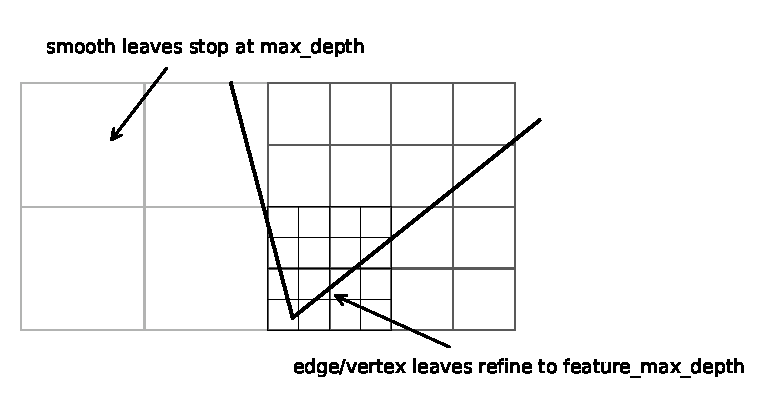
\includegraphics[width=0.90\textwidth]{fig_refinement.pdf}
\caption{Feature-specific refinement. Smooth leaves stop at the ordinary depth once the jet is accurate. Leaves containing edge, vertex or multi-sector behavior are allowed to refine more deeply.}
\label{fig:refinement}
\end{figure}

\subsection{Consistency certificates}

Each smooth leaf stores a certificate used to decide whether the smooth jet is valid:
\begin{enumerate}[label=(C\arabic*), leftmargin=1.8em]
\item the reference closest point is unique at the tested samples;
\item the active chart is constant over the leaf samples;
\item the closest point remains away from chart boundaries;
\item the normal-coordinate map is not close to singularity, i.e.
\begin{equation}
 \abs{1-d\kappa_a} \geq \gamma_\kappa>0,
 \qquad a=1,2;
\end{equation}
\item the stored jet errors $\eta_g$ and $\eta_n$ are below tolerance.
\end{enumerate}
If any of these certificates fail and the leaf cannot be refined further, the leaf is marked as multi-sector or invalid. A production solver may use a fallback projection or conservative primitive contact for invalid leaves. The prototype marks such leaves as multi-feature records.

\begin{proposition}[Runtime cost]
Assume the atlas lookup map returns a leaf index in $O(1)$ expected time and that each leaf stores at most $m_{\max}$ sector records. Then a runtime query costs $O(1)$ for a smooth leaf and $O(m_{\max})$ for a nonsmooth leaf, excluding downstream contact-solver work.
\end{proposition}

\begin{proof}
The smooth evaluation consists of one lookup and a fixed number of vector operations in Eq.~\eqref{eq:second_order_jet}. The nonsmooth evaluation applies the same fixed polynomial or plane evaluation to each stored sector. The closest-feature search, projection iterations and candidate sorting have been performed offline.
\end{proof}

\section{Coupling to contact solvers}
\label{sec:solver}

\subsection{Rigid body transform}

For a rigid body, the atlas is stored in the body-local frame. Let the world pose be $(R,r)$ and let $x_W$ be a world-space query point. The body-local query is
\begin{equation}
 x_B = R^\T(x_W-r).
\end{equation}
The atlas returns local gap and normals. A smooth normal is transformed back as
\begin{equation}
 n_W=R n_B,
\end{equation}
while a Hessian transforms as
\begin{equation}
 H_W=R H_B R^\T.
\end{equation}
For edge or vertex records, all active sector normals are transformed in the same way.

\subsection{Smooth constraint Jacobian and stiffness}

Let a slave material point or marker have world position $x_s(q)$, where $q$ are generalized coordinates. In a smooth leaf, the gap is
\begin{equation}
 g(q)=\widehat\phi_L(x_s(q)).
\end{equation}
The contact Jacobian is
\begin{equation}
 J_c(q)=\frac{\partial g}{\partial q}=\widehat n_L(x_s(q))^\T \frac{\partial x_s}{\partial q}.
\label{eq:jacobian_smooth}
\end{equation}
The second variation contains the geometric Hessian term
\begin{equation}
 \delta^2 g = \delta x_s^\T \widehat H_L \delta x_s + \widehat n_L^\T \delta^2 x_s.
\label{eq:gap_second_variation}
\end{equation}
For a penalty law $f_n=k\langle -g\rangle_+$, the contribution to the tangent stiffness includes
\begin{equation}
 K_c \supset k\left( J_c^\T J_c + \langle -g\rangle_+ B^\T \widehat H_L B\right),
\label{eq:penalty_stiffness}
\end{equation}
where $B=\partial x_s/\partial q$. Equation~\eqref{eq:penalty_stiffness} is one reason contact-consistent Hessians are useful. A trilinear grid SDF provides a poor approximation of $H_L$.

\subsection{Nonsmooth multi-sector constraints}

In a feature leaf, the solver receives $m_L$ local constraints
\begin{equation}
 g_i(q)=g_{i,L}(x_s(q)), \qquad i=1,\ldots,m_L.
\end{equation}
A frictionless complementarity formulation uses
\begin{equation}
 0\leq \lambda_i \perp g_i(q)\geq0,\qquad i=1,\ldots,m_L.
\label{eq:feature_lcp}
\end{equation}
The normal contact force is
\begin{equation}
 f_c=\sum_i \lambda_i n_i,
\end{equation}
which belongs to the stored normal cone. Penalty and augmented-Lagrangian methods can use the same constraints independently or can activate a subset based on the most violated sector. The atlas does not prescribe the contact law; it supplies the contact geometry.

\subsection{Universality of the interface}

The query output Eq.~\eqref{eq:query_object} separates geometry from the solver. The same atlas can be coupled to:
\begin{itemize}[leftmargin=1.6em]
\item rigid multibody time stepping using LCP or NCP formulations;
\item penalty or augmented-Lagrangian finite element contact;
\item variational contact potentials that need a signed gap and normal;
\item hybrid solvers that use projection fallback only when the atlas certificate fails;
\item CAD-derived, analytic, high-order finite element or ordinary mesh geometries, provided their contact geometry can be converted to normal sectors and local records.
\end{itemize}
This generality is an explicit design objective. The atlas is not tied to a specific primitive pair or to a specific global discretization.

\section{Numerical validation}
\label{sec:numerical}

\subsection{Prototype implementation}

A Python prototype was implemented to validate the end-to-end concept. It is not optimized C++ and should be interpreted as a relative algorithmic comparison. The prototype supports:
\begin{enumerate}[label=(\arabic*), leftmargin=1.8em]
\item analytic generation of corner-normal meshes for smooth, sharp and mixed-feature benchmarks, including the ellipsoid, sphere, hexagonal prism, capped cylinder, cone and torus;
\item export of an RMD-like corner-normal mesh block, with one triangle and three corner normals per record;
\item scalar grid SDF baselines using trilinear and tricubic interpolation, with normals obtained from the corresponding interpolant gradient;
\item an online projection reference using candidate search and closest-feature projection on the mesh;
\item uniform, adaptive and feature-specific Contact-SDF Atlas construction;
\item runtime atlas lookup without online projection.
\end{enumerate}
The main three-geometry experiments use the same generic backend. Smooth leaves use local Hessian jets when a unique smooth contact sector is credible, whereas feature leaves store normal-sector records and omit smooth curvature terms. A supplemental sphere test directly reports Hessian RMSE against the exact SDF Hessian.

The three analytic geometries are selected to isolate different behaviors. The ellipsoid is smooth and tests curvature. The hexagonal prism has planar faces and sharp edges/vertices. The cone has a smooth side surface, a sharp base rim and a singular apex. For the ellipsoid, analytic normals are
\begin{equation}
 n(x,y,z)=\frac{(x/a^2,y/b^2,z/c^2)}{\norm{(x/a^2,y/b^2,z/c^2)}}.
\end{equation}
For the prism and cone, the same geometric position can have different corner normals on different incident faces or sectors.

\subsection{Surface-based contact-error maps}

Before reporting aggregate errors, Figure~\ref{fig:surface_error_main} and Figure~\ref{fig:surface_error_supplemental} provide a qualitative check on the same geometric support. All methods are drawn on the original input triangle surface; only the face color changes. This avoids comparing the visual smoothness of different zero-level extraction procedures. Face colors report the absolute gap error and normal angular error at triangle face centers relative to the online corner-normal projection reference. For sharp-feature diagnostics, the methods are additionally evaluated at stored corner-normal sectors; red dots mark sharp-sector corners where the returned normal set misses the reference sector by more than $7.5^{\circ}$.

\begin{figure}[htbp]
\centering
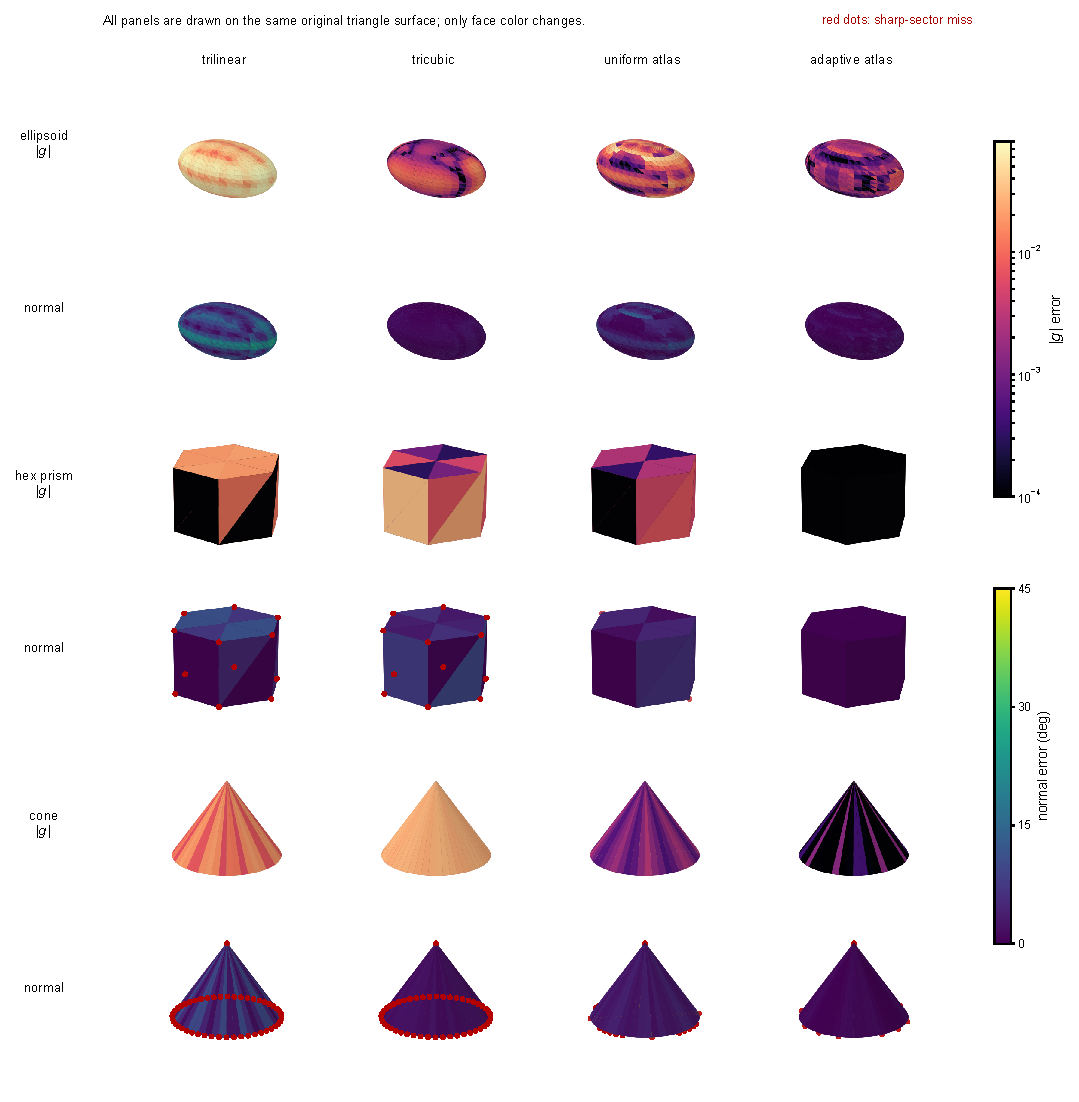
\includegraphics[width=0.98\textwidth]{fig_surface_error_main.pdf}
\caption{Surface-based contact-error maps for the three main benchmark bodies. Every panel uses the same original triangle surface for a given body, so apparent smoothness of an interpolated zero level set is not used as evidence. The upper row for each body shows $\abs{g}$ error on a logarithmic color scale; the lower row shows normal angular error. Red dots indicate missed sharp normal-sector constraints.}
\label{fig:surface_error_main}
\end{figure}

\begin{figure}[htbp]
\centering
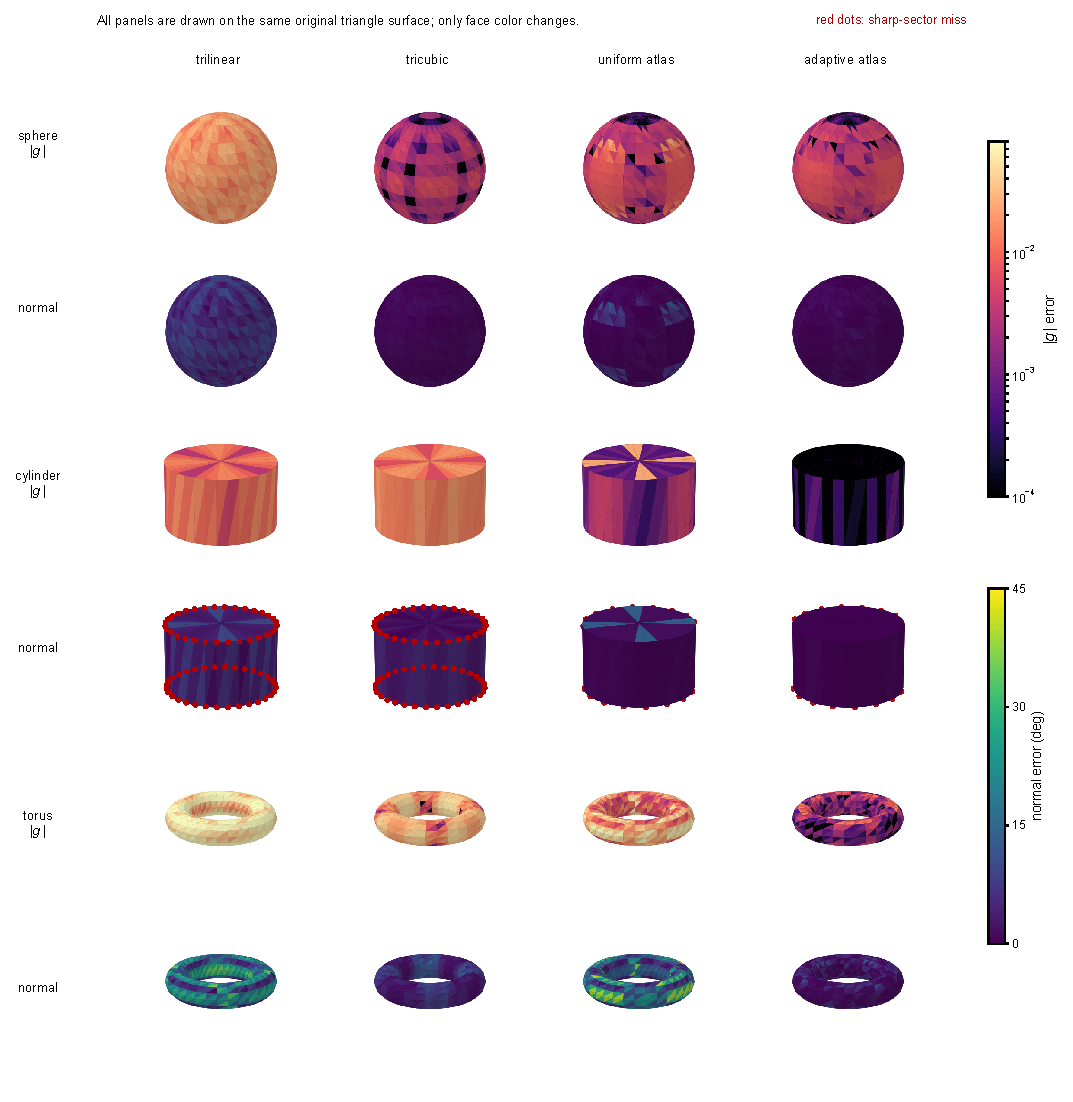
\includegraphics[width=0.98\textwidth]{fig_surface_error_supplemental.pdf}
\caption{Surface-based contact-error maps for supplemental benchmark bodies. The visualization protocol is identical to Figure~\ref{fig:surface_error_main}: common original surface geometry, face-center gap and normal errors, and red-dot markers for missed sharp-sector corners.}
\label{fig:surface_error_supplemental}
\end{figure}

\subsection{Industrial RMD representative geometries}

To check the same representation on imported industrial-style data, we also parse RecurDyn RMD surface blocks into the corner-normal triangle format used by the backend. The parsed inventory contains fifteen surface blocks, but several are near-duplicates: repeated ellipsoids, paired gears and related CSG-subtract bodies. Figure~\ref{fig:rmd_representatives} therefore shows a category-balanced subset rather than all parsed surfaces. The five selected representatives cover a smooth ellipsoid, a capped cylinder with sharp rims, a toothed gear, a grooved CSG solid and a sharp box-like polyhedron.

\begin{figure}[htbp]
\centering
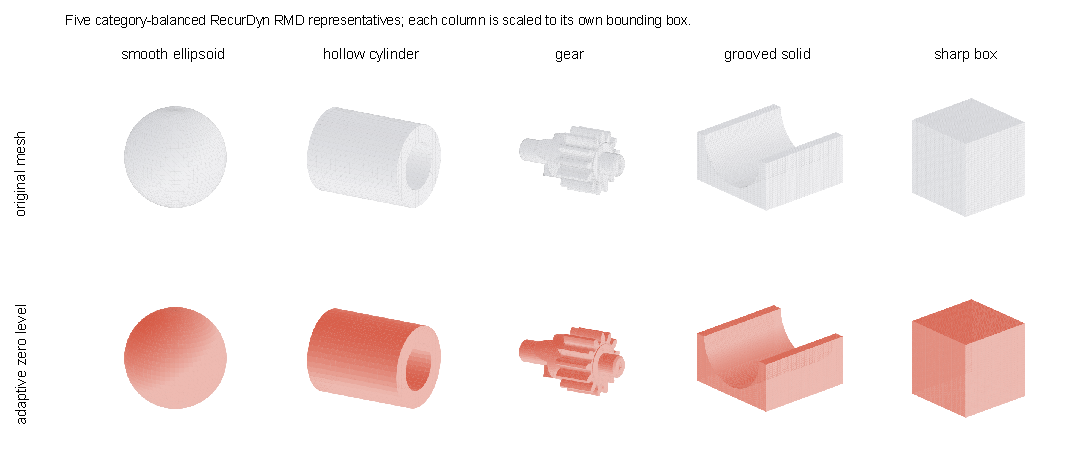
\includegraphics[width=0.98\textwidth]{fig_rmd_representatives.pdf}
\caption{Category-balanced RMD representatives selected from the parsed inventory. The upper row shows the original imported triangle meshes and the lower row shows the feature-adaptive atlas zero-level surface rendered with the same camera for each column. Each column is scaled to its own bounding box so that geometry type and feature coverage are visible; scale is not compared across columns.}
\label{fig:rmd_representatives}
\end{figure}

\subsection{Baselines and metrics}

Four representations are compared:
\begin{enumerate}[label=(B\arabic*), leftmargin=1.8em]
\item \textbf{Scalar grid SDFs}: scalar signed distances sampled on a grid, evaluated either by trilinear interpolation or by tricubic interpolation; normals are normalized gradients of the corresponding scalar interpolant.
\item \textbf{Uniform Contact-SDF Atlas}: fixed-depth atlas leaves storing smooth jets or multi-sector records.
\item \textbf{Feature-adaptive Contact-SDF Atlas}: smooth leaves and feature leaves refined with separate depth limits.
\item \textbf{Online projection reference}: runtime closest-feature search and projection, used as a timing and accuracy reference.
\end{enumerate}

The metrics are gap root-mean-square error (RMSE), mean normal angular error, normal-cone hit rate for sharp models, offline construction time and average microseconds per query. Gap and normal errors are computed against the online corner-normal projection baseline on the same tessellated mesh. The normal-cone hit rate is the fraction of normal-sector sharp-feature queries for which the returned sector set contains a reference-compatible normal sector. Plain point-to-triangle edge or vertex regions on an otherwise smooth benchmark are not counted as sharp-feature queries. Runtime timings use batch query interfaces for all grid and atlas representations; the atlas diagnostic interface that returns Python candidate lists is not used for the solver-facing query timing.

\subsection{Results}

Figure~\ref{fig:surface_error_main} gives the surface-local error evidence, Figure~\ref{fig:results} summarizes the aggregate trends and Table~\ref{tab:main_results} reports the corresponding values. Tricubic interpolation improves the scalar SDF over trilinear interpolation, especially on the smooth ellipsoid, but it remains a single scalar field and therefore cannot represent normal-sector alternatives at sharp features. The feature-adaptive atlas gives the lowest gap RMSE and mean normal error on all three bodies. On the ellipsoid, this improvement comes from the smooth second-order jet and Hessian-based normal update. On the sharp prism and cone, it comes from additional feature leaves and stored candidate sectors around normal-sector transitions.

\begin{table}[htbp]
\centering
\caption{Main geometric evidence. Arrows indicate the preferred direction; cone-hit is reported only for physical sharp-feature queries.}
\label{tab:main_results}
\resizebox{\textwidth}{!}{%
\begin{tabular}{lrrrrrrrrrr}
\toprule
Shape & \multicolumn{4}{c}{gap RMSE $\downarrow$} & \multicolumn{4}{c}{mean normal error $\downarrow$ (deg)} & \multicolumn{2}{c}{cone hit $\uparrow$}\\
\cmidrule(lr){2-5}\cmidrule(lr){6-9}\cmidrule(lr){10-11}
 & trilinear & tricubic & uniform & adaptive & trilinear & tricubic & uniform & adaptive & uniform & adaptive\\
\midrule
Ellipsoid & 0.0378 & 0.0186 & 0.0206 & \textbf{0.0116} & 10.68 & 3.32 & 3.76 & \textbf{1.43} & n/a & n/a\\
Hexagonal prism & 0.0477 & 0.0286 & 0.0396 & \textbf{0.0140} & 20.77 & 18.77 & 14.34 & \textbf{3.39} & 0.677 & \textbf{0.923}\\
Cone & 0.0431 & 0.0368 & 0.0382 & \textbf{0.0282} & 34.81 & 25.25 & 21.04 & \textbf{8.86} & 0.554 & \textbf{0.846}\\
\bottomrule
\end{tabular}}

\end{table}

The normal-cone hit rate increases from 0.677 to 0.923 on the prism and from 0.554 to 0.846 on the cone when feature-specific refinement is enabled. The smooth ellipsoid has no physical normal-sector feature, so its cone-hit field is not applicable. With vectorized batch query code, adaptive atlas lookup is sub-microsecond per query and remains comparable to trilinear scalar lookup while returning contact records rather than only a scalar-field gradient.

Table~\ref{tab:build_query_results} separates offline construction cost from query cost. The scalar trilinear and tricubic baselines share the same scalar signed-distance samples, so their construction times are nearly identical; tricubic pays primarily at query time because it evaluates a larger interpolation stencil. The feature-adaptive atlas has a much higher construction cost because it performs offline projection, refinement checks and feature-sector enrichment. The last column reports the approximate number of online-projection queries needed to amortize adaptive atlas construction.

\begin{table}[htbp]
\centering
\caption{Construction and query profile. Construction is reported in seconds, query time in microseconds per query, and break-even counts in thousands of online-projection queries.}
\label{tab:build_query_results}
\resizebox{\textwidth}{!}{%
\begin{tabular}{lrrrrrrrrrr}
\toprule
Shape & \multicolumn{4}{c}{construction (s)} & \multicolumn{5}{c}{query ($\mu$s)} & break-even\\
\cmidrule(lr){2-5}\cmidrule(lr){6-10}\cmidrule(lr){11-11}
 & trilinear & tricubic & uniform & adaptive & projection & trilinear & tricubic & uniform & adaptive & (k queries)\\
\midrule
Ellipsoid & 0.432 & 0.432 & 0.313 & 18.415 & 442.26 & 0.705 & 3.893 & 0.631 & \textbf{0.566} & 41.7\\
Hexagonal prism & 0.328 & 0.328 & 0.224 & 73.254 & 343.56 & 0.517 & 3.488 & 0.478 & \textbf{0.433} & 213.5\\
Cone & 0.423 & 0.423 & 0.290 & 70.665 & 364.27 & 0.505 & 3.516 & 0.476 & \textbf{0.444} & 194.2\\
\bottomrule
\end{tabular}}
\end{table}

\begin{figure}[htbp]
\centering
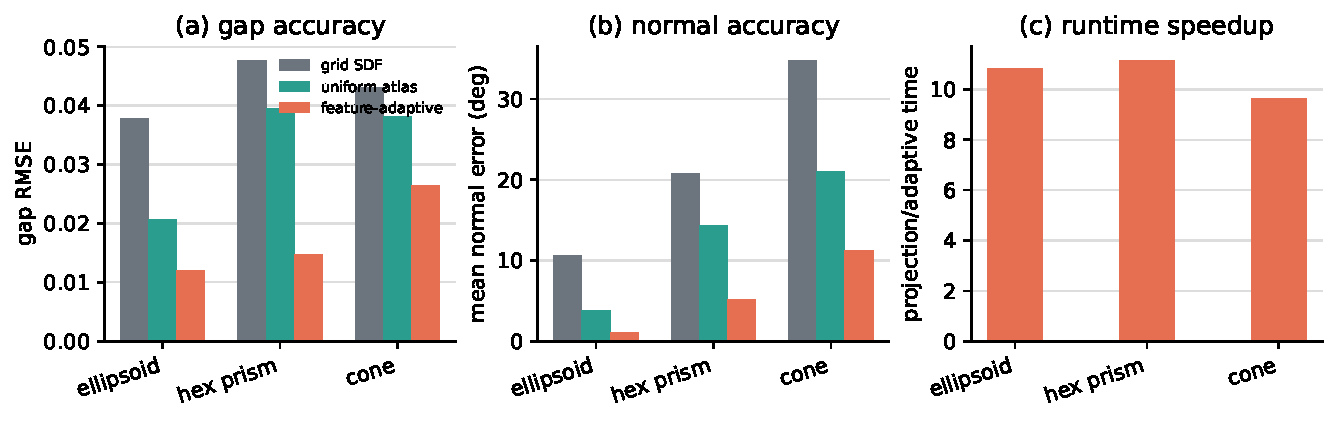
\includegraphics[width=0.95\textwidth]{fig_results.pdf}
\caption{Prototype results as a reviewer-facing evidence summary. (a) Mean contact-normal error. (b) Gap RMSE. (c) Normal-cone hit rate on sharp-feature queries. (d) Log-scale compact query time for online projection, scalar SDFs and the feature-adaptive atlas.}
\label{fig:results}
\end{figure}

\subsection{Supplemental geometric validation}

The supplemental validation suite checks whether the same generic backend behaves consistently beyond the three main geometries. No supplemental case uses case-specific runtime logic: the same projection reference, normal-sector extraction, uniform atlas and feature-adaptive atlas builders are used throughout. Figure~\ref{fig:surface_error_supplemental} gives the corresponding surface-local error maps. Table~\ref{tab:supplemental_results} is organized as a reviewer-risk audit: each row states the concern being tested, the key quantitative evidence and the conclusion supported by that evidence. Figure~\ref{fig:supplemental_validation} then shows the corresponding trends for exact smooth tests, feature-zone subsets, ablations, mesh refinements and noisy-normal stress tests. The automated advantage audit reports no failed checks.

\begin{table}[htbp]
\centering
\caption{Supplemental validation audit. Numeric pairs are uniform atlas $\rightarrow$ feature-adaptive atlas unless stated otherwise.}
\label{tab:supplemental_results}
{\footnotesize
\setlength{\tabcolsep}{4pt}
\renewcommand{\arraystretch}{0.94}
\begin{tabularx}{\textwidth}{@{}>{\raggedright\arraybackslash}p{0.18\textwidth}>{\raggedright\arraybackslash}p{0.50\textwidth}>{\raggedright\arraybackslash}X@{}}
\toprule
Reviewer concern & Key evidence & Conclusion\\
\midrule
Smooth jets &
Exact sphere: mean normal error $1.327\rightarrow\mathbf{0.527}$ deg; Hessian RMSE $0.527\rightarrow\mathbf{0.219}$. &
The normal and Hessian records are checked against exact SDF quantities.\\
Sharp sectors &
Capped-cylinder rim cone-hit $0.543\rightarrow\mathbf{0.914}$. &
The backend preserves edge and rim sectors instead of averaging them into one normal.\\
Cone zones &
Cone zones: side normal error $7.997\rightarrow\mathbf{3.822}$ deg; rim cone-hit $0.662\rightarrow\mathbf{0.926}$; apex cone-hit $0.246\rightarrow\mathbf{0.492}$. &
Generic feature handling improves side, rim and apex behavior; the apex remains singular.\\
Robustness &
Torus normal error $14.055\rightarrow\mathbf{1.383}$ deg; Fig.~\ref{fig:supplemental_validation} reports ablation and mesh-consistency trends; rigid-transform differences are $2.5{\times}10^{-16}$ gap and $2.2{\times}10^{-16}$ normal. &
The trend is not limited to convex shapes, one grid depth, one tessellation or one frame.\\
Limitation &
Noisy sphere normals at 10 deg: mean normal error $7.71\rightarrow8.48$ deg. &
Hessian fitting can amplify noisy visual normals and needs input-normal quality control.\\
\bottomrule
\end{tabularx}
}
\end{table}

The supplemental results support the same claims as the main tests. The smooth-jet and robustness rows show that the method is not limited to ellipsoids. The sharp-sector and cone-zone rows show that edge, rim and apex sectors are handled by the same normal-sector backend. Figure~\ref{fig:supplemental_validation} adds the ablation and mesh-consistency trends, showing that the advantage does not depend on a single resolution choice. The noisy-normal row is intentionally not highlighted as a win: it records that finite-difference Hessian estimates amplify input normal noise and should be paired with normal-quality controls for scanned or imported meshes.

\begin{figure}[htbp]
\centering
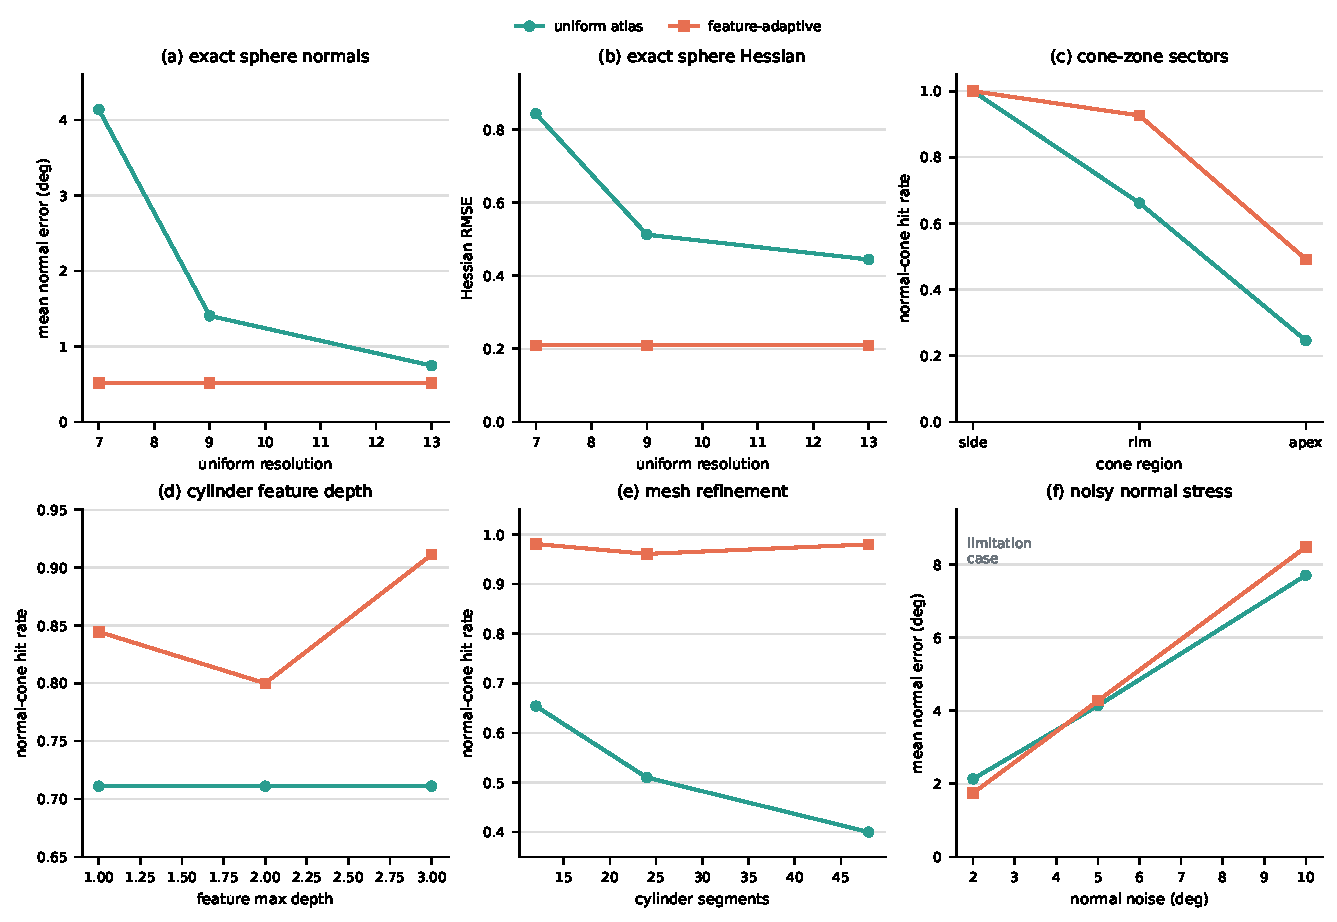
\includegraphics[width=0.98\textwidth]{fig_supplemental_validation.pdf}
\caption{Supplemental validation trends. (a) Exact sphere normal error across grid resolutions. (b) Exact sphere Hessian RMSE. (c) Cone side, rim and apex normal-sector hit rates. (d) Cylinder feature-depth ablation. (e) Cylinder mesh-refinement consistency. (f) Noisy-normal stress test, retained as a limitation case rather than an advantage claim.}
\label{fig:supplemental_validation}
\end{figure}

\subsection{Interpretation}

The results support three observations. First, a scalar grid SDF is not sufficient when contact normals are important. Tricubic interpolation improves scalar-field smoothness relative to trilinear interpolation, but both baselines still return a single interpolant gradient and cannot preserve normal sectors or singular features. Second, storing local contact records improves the quantities that contact solvers actually use. Smooth jets improve curvature-sensitive normals, while feature records preserve multi-normal behavior. Figure~\ref{fig:supplemental_validation} shows that these trends persist across exact smooth references, feature-zone subsets and mesh refinements. Third, moving projection offline changes the cost profile: atlas construction is more expensive, especially for feature-adaptive refinement, but compact runtime lookup avoids per-query projection and remains comparable to scalar-grid lookup in the batch Python backend.

The cone remains the most difficult case. Its apex is a true singular point, so no smooth normal or Hessian exists there. The feature-specific atlas improves mean normal error and cone-hit rate, and the apex-zone row in Table~\ref{tab:supplemental_results} confirms that welded-vertex sector exposure improves apex cone-hit rate without cone-specific logic. The highest-percentile cone errors can still be large near singular transitions, which is expected for a compact finite-sector leaf record and should be treated as a resolution/storage trade-off when apex contact is critical.

\section{Discussion: generality, accuracy and limitations}
\label{sec:discussion}

\subsection{Generality across geometry sources}

Although the implementation in this paper uses corner-normal triangle meshes, the mathematical object is more general. The atlas needs a finite set of local contact records. These records can be generated from different sources:
\begin{itemize}[leftmargin=1.6em]
\item \textbf{Analytic primitives}: exact normals, curvatures and feature cones can be baked directly.
\item \textbf{CAD boundary representations}: faces, trims, edges and vertices already define a stratified feature complex; tessellation can be used only for acceleration, while local records may come from CAD projection and CAD curvature.
\item \textbf{Corner-normal engineering meshes}: the current target format; discontinuous face-corner normals define normal sectors.
\item \textbf{Plain triangle meshes}: face normals define a conservative piecewise-linear contact atlas; high-order jets should not be claimed unless additional reconstruction is performed.
\item \textbf{High-order finite element or isogeometric boundaries}: element patches can provide smooth local geometry and curvature derivatives.
\end{itemize}
Thus the Contact-SDF Atlas is best viewed as a common contact-geometry storage layer. The fidelity of the record is limited by the fidelity of the source geometry.

\subsection{Relation to scalar SDFs}

The proposed atlas is not a replacement for all scalar SDF uses. Scalar SDFs remain excellent for broadphase culling, approximate penetration queries and rendering. The distinction is that contact simulation needs derivatives and feature information. A scalar sampled SDF stores one number per grid node, whereas the atlas stores a local model. In smooth regions, this model approximates the distance jet; at nonsmooth features, it stores a set of active sector constraints. This is why the atlas can preserve sharp normal behavior that a scalar interpolant tends to smear.

\subsection{Accuracy limitations}

The method does not provide exact geometry for arbitrary input meshes. If the source is a coarse mesh, the atlas is only as accurate as the mesh and corner normals. If the corner normals are visual smoothing normals that ignore real hard edges, the normal-sector detection may need correction. If the body undergoes large deformation, a rigidly stored atlas will no longer match the current boundary; one then needs either local atlas updates, reference-to-current deformation correction or fallback projection. If global nonpenetration guarantees are required, the atlas must be coupled to an appropriate time-stepping, complementarity, barrier or continuous-collision framework. The atlas provides contact geometry; it is not by itself a complete nonpenetration solver.

\subsection{When the method is most useful}

The expected advantage is largest when the same body is queried many times and when contact normals affect dynamics strongly. Examples include gears, cams, bearings, clearance joints, rigid bodies with high-resolution engineering surfaces, and repeated contact search in multibody dynamics. In such cases, projection can be amortized offline, and preserving normal sectors can reduce nonphysical smoothing at sharp features.

\section{Conclusions}
\label{sec:conclusion}

This paper introduced a feature-aware Contact-SDF Atlas for fast and consistent contact geometry queries from corner-normal triangle meshes. The central idea is to store contact-ready local records instead of scalar distance samples. Smooth leaves store signed-distance jets derived from closest-point geometry, with optional Hessian support, while sharp edge and vertex leaves store active normal-sector models and normal cones. A feature-specific adaptive refinement strategy concentrates resolution near nonsmooth contact features. Runtime queries perform lookup and polynomial or multi-sector evaluation, avoiding closest-point projection during time stepping.

Theoretical derivations show that, in smooth regions, the SDF gradient and Hessian are determined by the closest-point normal and curvature, not by an interpolation basis. At sharp features, the appropriate object is a normal cone rather than a single averaged normal. Prototype benchmarks on analytic smooth and nonsmooth bodies show improved contact-normal consistency compared with scalar trilinear and tricubic SDFs. The separated cost measurements show the expected trade-off: adaptive atlas construction is more expensive, but compact runtime queries are sub-microsecond in the batch Python backend and avoid online projection. Supplemental sphere tests exercise the Hessian error directly, while robust Hessian estimation for noisy imported normals remains future work. The formulation is solver-agnostic and can be coupled to common contact algorithms in multibody dynamics and finite element analysis.

Future work will extend the prototype in four directions: a production parser for industrial corner-normal formats; exact CAD-backed records for B-rep features; analytic feature records for singular primitives such as cone apices; and dynamic benchmarks in which contact force, energy, constraint violation and runtime are compared against projection-based and scalar-SDF baselines.

\section*{CRediT authorship contribution statement}
Sohansome Body: Conceptualization, Methodology, Software, Validation, Writing - original draft. Second Author: Supervision, Writing - review and editing. Third Author: Validation, Writing - review and editing. This section is a placeholder and should be edited before submission.

\section*{Declaration of competing interest}
The authors declare that they have no known competing financial interests or personal relationships that could have appeared to influence the work reported in this paper. This statement is a placeholder and should be verified before submission.

\section*{Declaration of generative AI and AI-assisted technologies in the writing process}
During preparation of this draft, AI-assisted language tools were used to help generate and organize manuscript text. The authors are responsible for reviewing, editing and verifying all scientific content before submission. This statement should be revised according to the final journal policy and actual author workflow.

\section*{Data availability}
The prototype code, manuscript source and generated benchmark data are available at \url{https://github.com/W-Moorer/contact-sdf-dynamics}. The repository includes the scripts used to generate the tabulated validation metrics.

\section*{Acknowledgements}
The authors acknowledge discussions on signed-distance contact representations, corner-normal meshes and multibody contact simulation. Funding information should be inserted here.

\appendix

\section{Appendix A. Derivation of the Hessian formula}
\label{app:hessian}

Let $p=r(u)$ and $x=p+d n(p)$. Let $\tau\in T_p\Gamma$ be a tangent vector. The differential of the offset map $\Psi(p,d)=p+d n(p)$ is
\begin{equation}
 D\Psi[\tau] = \tau+dD_\tau n = \tau-dS\tau=(I-dS)\tau.
\end{equation}
For a spatial displacement $\xi$ tangent to the offset surface, the corresponding tangent displacement on the base surface is
\begin{equation}
 \tau=(I-dS)^{-1}\xi_T,
\end{equation}
where $\xi_T=P_T\xi$. Since $\nabla\phi=n$, the Hessian satisfies
\begin{equation}
 \nabla^2\phi\,\xi = D_\xi n = D_\tau n = -S\tau = -S(I-dS)^{-1}P_T\xi.
\end{equation}
This proves Eq.~\eqref{eq:hessian_operator}. Local invertibility requires $1-d\kappa_a\neq0$ for both principal curvatures.

\section{Appendix B. Analytic benchmark generation}
\label{app:benchmarks}

\subsection{Ellipsoid}

The ellipsoid is
\begin{equation}
 \frac{x^2}{a^2}+\frac{y^2}{b^2}+\frac{z^2}{c^2}=1.
\end{equation}
A vertex on the triangulated ellipsoid has analytic normal
\begin{equation}
 n = \frac{(x/a^2,y/b^2,z/c^2)}{\norm{(x/a^2,y/b^2,z/c^2)}}.
\end{equation}
All incident corner normals are continuous up to tessellation error, so the normal-sector complex contains smooth charts and no physical sharp edges.

\subsection{Hexagonal prism}

The prism is generated from a regular hexagon extruded along the $z$ axis. Each side face, top face and bottom face assigns its own constant corner normal. The same geometric vertex appears with multiple face-corner normals. Therefore all vertical edges and top/bottom rim edges are sharp normal-sector features.

\subsection{Cone}

The cone has a circular base and an apex. The side surface assigns the analytic cone-side normal, the base assigns the base normal, and the apex stores multiple side-sector normals. The base rim and apex are nonsmooth. The apex does not have a unique tangent plane, so it is represented by a normal fan rather than by a smooth SDF jet.

\section{Appendix C. Suggested dynamic validation cases}
\label{app:dynamic}

For a full CMAME submission, static geometric metrics should be complemented by dynamic tests. Recommended cases are:
\begin{enumerate}[leftmargin=1.8em]
\item \textbf{Sphere/ellipsoid sliding on a curved track}: verifies smooth-jet normals and curvature-sensitive stiffness.
\item \textbf{Prism edge impact}: verifies normal-cone contact and absence of artificial averaged normals.
\item \textbf{Cone apex/rim impact}: stresses singular feature handling and multi-sector constraints.
\item \textbf{Gear-like tooth contact}: demonstrates relevance to engineering multibody models with sharp and smooth features.
\item \textbf{Clearance joint}: measures gap, force, acceleration and energy sensitivity to contact-normal errors.
\end{enumerate}
For each case the recommended outputs are gap history, active feature history, contact-normal jump, contact force, kinetic and total energy, constraint violation and wall-clock time.

\bibliographystyle{elsarticle-num}
\bibliography{references}

\end{document}
